% This file was created by matlab2tikz.
%
%The latest updates can be retrieved from
%  http://www.mathworks.com/matlabcentral/fileexchange/22022-matlab2tikz-matlab2tikz
%where you can also make suggestions and rate matlab2tikz.
%
\definecolor{mycolor1}{rgb}{0.00000,0.44700,0.74100}%
\definecolor{mycolor2}{rgb}{0.85000,0.32500,0.09800}%
\definecolor{mycolor3}{rgb}{0.92900,0.69400,0.12500}%
\definecolor{mycolor4}{rgb}{0.49400,0.18400,0.55600}%
%
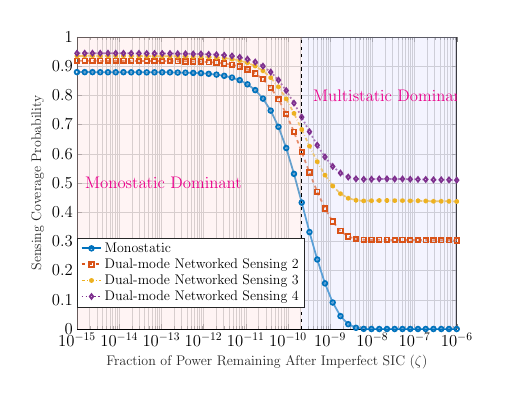
\begin{tikzpicture}[scale=0.42, transform shape,font=\Large]

\begin{axis}[%
width=4.521in,
height=3.477in,
at={(0.758in,0.57in)},
scale only axis,
xmode=log,
xmin=1e-15,
xmax=1e-06,
xminorticks=true,
xlabel style={font=\large\color{white!15!black}},
xlabel={Fraction of Power Remaining After Imperfect SIC $(\zeta)$},
ymin=0,
ymax=1,
ylabel style={font=\large\color{white!15!black}},
ylabel={Sensing Coverage Probability},
axis background/.style={fill=white},
xmajorgrids,
xminorgrids,
ymajorgrids,
legend style={at={(0,0.075)}, anchor=south west, legend cell align=left, align=left, draw=white!15!black, font=\large}
]
\addplot [color=mycolor1, line width=1.5pt, mark=o, mark options={solid, mycolor1}]
  table[row sep=crcr]{%
1e-06	0\\
6.55128556859551e-07	0\\
4.29193426012878e-07	0\\
2.81176869797423e-07	0\\
1.84206996932672e-07	0\\
1.20679264063933e-07	0\\
7.9060432109077e-08	0\\
5.17947467923121e-08	0\\
3.39322177189533e-08	0\\
2.2229964825262e-08	0\\
1.45634847750124e-08	0\\
9.54095476349996e-09	2.85714285714286e-05\\
6.25055192527398e-09	0.0005\\
4.09491506238042e-09	0.0041\\
2.68269579527973e-09	0.0165285714285714\\
1.75751062485479e-09	0.0441142857142857\\
1.15139539932645e-09	0.0906428571428571\\
7.54312006335461e-10	0.156357142857143\\
4.94171336132384e-10	0.238085714285714\\
3.23745754281764e-10	0.331842857142857\\
2.12095088792019e-10	0.432914285714286\\
1.38949549437314e-10	0.531185714285714\\
9.10298177991523e-11	0.619714285714286\\
5.96362331659466e-11	0.692214285714286\\
3.90693993705462e-11	0.747785714285714\\
2.55954792269953e-11	0.788857142857143\\
1.676832936811e-11	0.817971428571428\\
1.09854114198756e-11	0.8378\\
7.19685673001153e-12	0.852028571428571\\
4.71486636345739e-12	0.860771428571429\\
3.08884359647747e-12	0.866871428571429\\
2.02358964772516e-12	0.870985714285714\\
1.32571136559011e-12	0.873642857142857\\
8.68511373751352e-13	0.875957142857143\\
5.68986602901828e-13	0.876785714285714\\
3.72759372031494e-13	0.877485714285714\\
2.44205309454866e-13	0.878028571428571\\
1.59985871960606e-13	0.878828571428571\\
1.04811313415468e-13	0.8789\\
6.866488450043e-14	0.878928571428571\\
4.49843266896945e-14	0.878614285714286\\
2.94705170255181e-14	0.878928571428571\\
1.93069772888325e-14	0.8789\\
1.2648552168553e-14	0.879328571428571\\
8.28642772854686e-15	0.879\\
5.42867543932386e-15	0.879128571428571\\
3.55648030622314e-15	0.879228571428571\\
2.32995181051537e-15	0.879533333333333\\
1.52641796717524e-15	0.87954\\
1e-15	0.879625\\
};
\addlegendentry{Monostatic}

\addplot [color=mycolor2, dashed, line width=1.5pt, mark=square, mark options={solid, mycolor2}]
  table[row sep=crcr]{%
1e-06	0.303625\\
6.55128556859551e-07	0.30446\\
4.29193426012878e-07	0.3043\\
2.81176869797423e-07	0.304071428571429\\
1.84206996932672e-07	0.304571428571429\\
1.20679264063933e-07	0.304671428571429\\
7.9060432109077e-08	0.304614285714286\\
5.17947467923121e-08	0.304971428571429\\
3.39322177189533e-08	0.304814285714286\\
2.2229964825262e-08	0.305171428571429\\
1.45634847750124e-08	0.305471428571429\\
9.54095476349996e-09	0.305057142857143\\
6.25055192527398e-09	0.305314285714286\\
4.09491506238042e-09	0.308042857142857\\
2.68269579527973e-09	0.316385714285714\\
1.75751062485479e-09	0.335728571428571\\
1.15139539932645e-09	0.367714285714286\\
7.54312006335461e-10	0.4132\\
4.94171336132384e-10	0.469857142857143\\
3.23745754281764e-10	0.535471428571429\\
2.12095088792019e-10	0.605971428571428\\
1.38949549437314e-10	0.674714285714286\\
9.10298177991523e-11	0.736085714285714\\
5.96362331659466e-11	0.787028571428571\\
3.90693993705462e-11	0.826185714285714\\
2.55954792269953e-11	0.855042857142857\\
1.676832936811e-11	0.875042857142857\\
1.09854114198756e-11	0.888842857142857\\
7.19685673001153e-12	0.898814285714286\\
4.71486636345739e-12	0.904885714285714\\
3.08884359647747e-12	0.909028571428571\\
2.02358964772516e-12	0.9119\\
1.32571136559011e-12	0.913757142857143\\
8.68511373751352e-13	0.9156\\
5.68986602901828e-13	0.915914285714286\\
3.72759372031494e-13	0.9165\\
2.44205309454866e-13	0.917\\
1.59985871960606e-13	0.917585714285714\\
1.04811313415468e-13	0.917671428571429\\
6.866488450043e-14	0.917614285714286\\
4.49843266896945e-14	0.9175\\
2.94705170255181e-14	0.917757142857143\\
1.93069772888325e-14	0.917857142857143\\
1.2648552168553e-14	0.917985714285714\\
8.28642772854686e-15	0.917828571428571\\
5.42867543932386e-15	0.917842857142857\\
3.55648030622314e-15	0.918042857142857\\
2.32995181051537e-15	0.9182\\
1.52641796717524e-15	0.91842\\
1e-15	0.91825\\
};
\addlegendentry{Dual-mode Networked Sensing 2}

\addplot [color=mycolor3, dashdotted, line width=1.5pt, mark=asterisk, mark options={solid, mycolor3}]
  table[row sep=crcr]{%
1e-06	0.43665\\
6.55128556859551e-07	0.4375\\
4.29193426012878e-07	0.43735\\
2.81176869797423e-07	0.437285714285714\\
1.84206996932672e-07	0.4383\\
1.20679264063933e-07	0.438942857142857\\
7.9060432109077e-08	0.438857142857143\\
5.17947467923121e-08	0.439642857142857\\
3.39322177189533e-08	0.439614285714286\\
2.2229964825262e-08	0.440071428571429\\
1.45634847750124e-08	0.439971428571429\\
9.54095476349996e-09	0.439128571428571\\
6.25055192527398e-09	0.438585714285714\\
4.09491506238042e-09	0.440814285714286\\
2.68269579527973e-09	0.4478\\
1.75751062485479e-09	0.463285714285714\\
1.15139539932645e-09	0.4895\\
7.54312006335461e-10	0.526814285714286\\
4.94171336132384e-10	0.572871428571428\\
3.23745754281764e-10	0.626014285714286\\
2.12095088792019e-10	0.683028571428571\\
1.38949549437314e-10	0.7383\\
9.10298177991523e-11	0.788\\
5.96362331659466e-11	0.828957142857143\\
3.90693993705462e-11	0.860528571428572\\
2.55954792269953e-11	0.883942857142857\\
1.676832936811e-11	0.900342857142857\\
1.09854114198756e-11	0.911471428571429\\
7.19685673001153e-12	0.9193\\
4.71486636345739e-12	0.924257142857143\\
3.08884359647747e-12	0.927371428571429\\
2.02358964772516e-12	0.929585714285714\\
1.32571136559011e-12	0.931014285714286\\
8.68511373751352e-13	0.932485714285714\\
5.68986602901828e-13	0.932685714285714\\
3.72759372031494e-13	0.9333\\
2.44205309454866e-13	0.933542857142857\\
1.59985871960606e-13	0.934085714285714\\
1.04811313415468e-13	0.934057142857143\\
6.866488450043e-14	0.934128571428571\\
4.49843266896945e-14	0.934057142857143\\
2.94705170255181e-14	0.934471428571429\\
1.93069772888325e-14	0.934628571428571\\
1.2648552168553e-14	0.934942857142857\\
8.28642772854686e-15	0.934957142857143\\
5.42867543932386e-15	0.935114285714286\\
3.55648030622314e-15	0.935014285714286\\
2.32995181051537e-15	0.935183333333333\\
1.52641796717524e-15	0.93518\\
1e-15	0.934975\\
};
\addlegendentry{Dual-mode Networked Sensing 3}

\addplot [color=mycolor4, dotted, line width=1.5pt, mark=diamond, mark options={solid, mycolor4}]
  table[row sep=crcr]{%
1e-06	0.509675\\
6.55128556859551e-07	0.51072\\
4.29193426012878e-07	0.5108\\
2.81176869797423e-07	0.510871428571429\\
1.84206996932672e-07	0.511942857142857\\
1.20679264063933e-07	0.512214285714286\\
7.9060432109077e-08	0.512728571428571\\
5.17947467923121e-08	0.513642857142857\\
3.39322177189533e-08	0.513414285714286\\
2.2229964825262e-08	0.514028571428571\\
1.45634847750124e-08	0.513885714285714\\
9.54095476349996e-09	0.512757142857143\\
6.25055192527398e-09	0.512557142857143\\
4.09491506238042e-09	0.514014285714286\\
2.68269579527973e-09	0.520314285714286\\
1.75751062485479e-09	0.534142857142857\\
1.15139539932645e-09	0.5566\\
7.54312006335461e-10	0.5891\\
4.94171336132384e-10	0.629371428571429\\
3.23745754281764e-10	0.6756\\
2.12095088792019e-10	0.725542857142857\\
1.38949549437314e-10	0.773528571428571\\
9.10298177991523e-11	0.816471428571429\\
5.96362331659466e-11	0.852242857142857\\
3.90693993705462e-11	0.879657142857143\\
2.55954792269953e-11	0.900014285714286\\
1.676832936811e-11	0.914171428571429\\
1.09854114198756e-11	0.923757142857143\\
7.19685673001153e-12	0.930457142857143\\
4.71486636345739e-12	0.934785714285714\\
3.08884359647747e-12	0.937271428571429\\
2.02358964772516e-12	0.939185714285714\\
1.32571136559011e-12	0.940371428571429\\
8.68511373751352e-13	0.941642857142857\\
5.68986602901828e-13	0.941814285714286\\
3.72759372031494e-13	0.942442857142857\\
2.44205309454866e-13	0.942628571428571\\
1.59985871960606e-13	0.943185714285714\\
1.04811313415468e-13	0.943085714285714\\
6.866488450043e-14	0.943242857142857\\
4.49843266896945e-14	0.943314285714286\\
2.94705170255181e-14	0.943642857142857\\
1.93069772888325e-14	0.943714285714286\\
1.2648552168553e-14	0.944028571428571\\
8.28642772854686e-15	0.944071428571429\\
5.42867543932386e-15	0.944271428571429\\
3.55648030622314e-15	0.944128571428571\\
2.32995181051537e-15	0.9442\\
1.52641796717524e-15	0.94418\\
1e-15	0.944\\
};
\addlegendentry{Dual-mode Networked Sensing 4}

  % Region A (light pink, left of dashed line)
    \addplot[fill=red!10, draw=none, fill opacity=0.4] 
        coordinates {(1e-15, 0) (2.12095088792019e-10, 0) (2.12095088792019e-10, 1) (1e-15, 1)} -- cycle;

    % Region B (light blue, right of dashed line)
    \addplot[fill=blue!10, draw=none, fill opacity=0.4] 
        coordinates {(2.12095088792019e-10, 0) (1e-6, 0) (1e-6, 1) (2.12095088792019e-10, 1)} -- cycle;

    % Vertical dashed line at x = 2.12095088792019e-10
    \addplot[thick, dashed, black] 
        coordinates {(2.12095088792019e-10, 0) (2.12095088792019e-10, 1)};

    % Labels for regions
   \node[anchor=east, text=magenta] at (axis cs:1e-11, 0.5) {Monostatic Dominant}; % Left region label
    \node[anchor=west, text=magenta] at (axis cs:3.162e-10, 0.8) {Multistatic Dominant};  % Right region label

\end{axis}



\end{tikzpicture}%